\documentclass[11pt]{report}
% packages
% Fran Burstall's Bath thesis package
\usepackage{baththesis}
\usepackage{amssymb} %for Blackboard bold etc \usepackage{graphicx} %for including eps graphics % front matter
\usepackage[pdftex]{graphicx} % To include pictures
\usepackage{caption}
\usepackage{subcaption} % To use subfigures with subcaptions
\usepackage{url}
\usepackage{amsmath} % Equations
\usepackage{txfonts}
\setlength{\parskip}{0.9em} %Paragraph spacing
\usepackage{pgfgantt}
\usepackage{cite}
\usepackage{csquotes}
\renewcommand*{\mkcitation}[1]{ #1}

\newcommand{\phim}{\mathbf{\phi}}
\newcommand{\X}{\mathbf{X}}
\newcommand{\x}{\mathbf{x}}
\newcommand{\w}{\mathbf{w}}
\newcommand{\Z}{\mathbf{Z}}
\newcommand{\z}{\mathbf{z}}
\newcommand{\h}{\mathbf{h}}

%\usepackage[hidelinks]{hyperref} % Adds references links without color
\usepackage{hyperref} % Adds references links with color
\usepackage{xcolor}
\hypersetup{
    colorlinks,
    linkcolor={red!50!black},
    citecolor={blue!50!black},
    urlcolor={blue!80!black}
}

\title{Visual Effects} \author{Ieva Kazlauskaite, Garoe Dorta-Perez, Richard Shaw}
%\degree{Doctor of Philosophy}
\unit{ unit }
\department{Department of Computer Sciences} \degreemonthyear{May 2015}
\norestrictions

\begin{document}
\maketitle

\chapter{Introduction}
\label{ch:intro}
\begin{center}
\textquote[~\cite{Attenborough:1998}]{\textit{Birds are the most accomplished aeronauts the world has ever seen. They fly high and low, at great speed, and very slowly. And always with extraordinary precision and control}.}
\end{center}


\chapter{Previous Work}
\label{sec:previous}

\section{Data Capture}


\section{Sparse Reconstruction}


\section{Blendshape Optimisation}


\section{Skin Rendering}

\begin{figure}[htbp!]
\centering
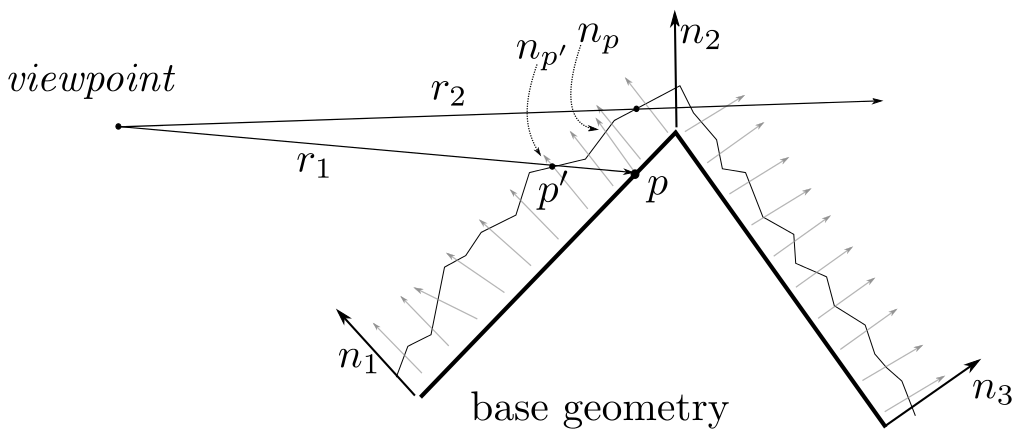
\includegraphics[width=0.7\textwidth]{img/normal_map}
	\caption{ Using normal maps to simplify a given geometry, image taken from \cite{ganovelli2014}.}
	\label{fig:normal_map}
\end{figure}



%-----------------------------------------------------------------------
\chapter{Methodology}
\label{sec:methods}


\section{Data Capture}


\section{Sparse Reconstruction}


\section{Blendshape Optimisation}


\section{Skin Rendering}


%-----------------------------------------------------------------------
\chapter{Results}


%-----------------------------------------------------------------------
\chapter{Conclusions}


\nocite{*}
\bibliographystyle{eg-alpha}
\bibliography{baththesis}

\end{document}